\newpage
\section{Описание организационной структуры}

Для дальнейшего ознакомления с предприятием мною была выдвинута инициатива по изучению документов таких как устав
с целью составления организационной структуры и составления примерного вида должностей.
Моей просьбе было отказано, так как это рассекречивание тайн компанию.
После чего менеджер Кристина сообщила, что в открытом доступе можно брать информацию с сайта.

После изучения сайта предприятия я не нашел, то что хотел, и мною была выдвинута инициатива идти общаться с директором.
В ходе общения с директором в городе Брест (хэд офиса) с устной речи мною были законспектировать следующие должности:

\begin{itemize}
  \item хэд офиса (директор, Ольга Крусь);
  \item офис менеджер (менеджер, Кристина Галаюк);
  \item практикант (студент, Галанин Павел);
  \item руководитель практики от предприятия (технический программист, Михаил Юдин);
  \item ментор (выделенные люди для вопросов по проекту);
  \item интерн (стажер с оплачиваемой стажировкой);
  \item транью (стажер с не оплачиваемой стажировкой);
  \item проджект менеджер (были два объекта женского пола);
  \item программисты:
  \begin{itemize}
    \item java отдел;
    \item python отдел;
    \item отдел мобильной разработки на Flutter;
    \item отдел мобильной разработки на iOS;
    \item отдел фронта на React;
    \item отдел фронта на VueJS.
  \end{itemize}
  \item тим лид (отвечающий за проект, которые обычно в Минске).
\end{itemize}

В связи с тем что большая часть спрятана в других городах, таких как город Витебс и город Минск и директором было сказано,
что тут только программисты, то мною была составлена следующая организационная структура
по городу Брест (см.~рис.~\ref{fig:OrganizationalChart}).

\begin{figure}[!ph]
  \centering

  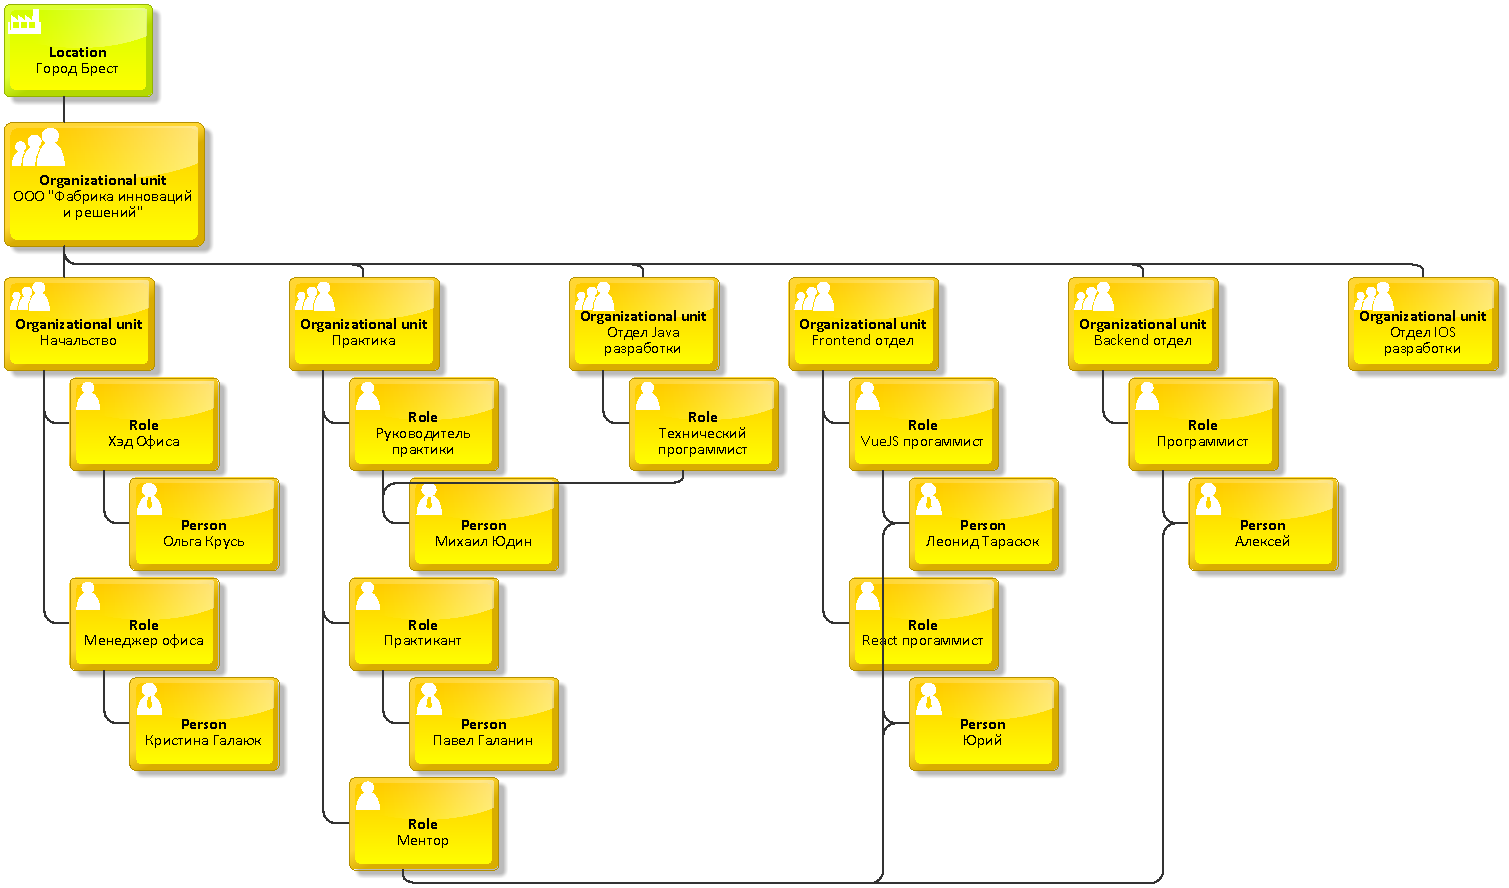
\includegraphics[width=16cm]
  {../design/ARIS/OrganizationalChart.adf.png}

  \caption{Организационная структура}
  \label{fig:OrganizationalChart}
\end{figure}

\begin{figure}[!ph]
  \centering

  \includegraphics[width=16cm]
  {../design/ARIS/export/ItDepartmentsDiagram-Page-1.pdf}

  \caption{Отрасли для программиста}
  \label{fig:ItDepartmentsDiagram}
\end{figure}


Для составления отделов по технологиям я ознакомился с сайтом предприятия \cite{InnowiseItDepartment}.

Cоотвествие с организационной структурой города Бреста я на сайте не наше,
и поэтому составил полную структуру IT-областей
(см.~рис.~\ref{fig:ItDepartmentsDiagram}).
